%\vspace{-5mm}
\section{Prototype Implementation}

We implemented the prototype of DASF on Android 4.1.1 (\textit{Jellybean}) and
TaintDroid.  We have also implemented a server program that utilizes our
message protocol to transfer data and dynamic privilege restrictions and
unrestrictions to DASF and applications running on our prototype.  
%We assume
%that DASF utilizes the CleanOS extension of TaintDroid, which
%provides a mechanism for revoking access to tainted data. However, our prototype
%is actually directly implemented over the TaintDroid platform because
%the source code for the CleanOS project was not available.  Regardless
%of that fact, our security model is designed to be easily integrated into
%the CleanOS architecture to take advantage of the data revocation
%mechanism that it offers.

%Specifically, the four sensitivity levels that our security model defines to
%enforce security policies on sensitive can can be defined as the
%highest sensitivity level of secure data objects on CleanOS.  Further,
%CleanOS' propagation logic would need to be modified to handle
%the escalating of sensitivity levels that correlate to security policies
%when combining data with different sensitivity levels as mentioned in
%our security model.  Also, the organization that sends the sensitive
%data to the device would need to control CleanOS' cloud service that is
%used for revoking sensitive data.  However, since we implement our prototype
%directly over TaintDroid, we emulate the sensitivity levels mentioned above
%by defining four custom privacy tags and enforce the system restrictions based
%off of those tags.

The architecture of the prototype of DASF consists of three modifications to
the Android platform and TaintDroid. First, we define the four privacy tags
mentioned in the previous section and place the hooks in the Java libraries to
enforce the security policies on sensitive data.  Second, a system service is
added to manage the dynamic system-wide privilege restrictions and place hooks
in the Android framework libraries to enforce the privilege restrictions.
Third, we design a new message protocol in the system to tag sensitive data
that is received from the server and modify the Java libraries to force
\textit{medical applications} to use our message protocol.

\subsection{Restriction Policy Manifest File}  
For applications to utilize DASF, the application must include a special
manifest file that is parsed during the application's installation.  As stated
in our security model, DASF allows applications to dynamically enforce
system-wide permission restrictions that may be programmatically set in an
application's code or by receiving messages from the trusted server using
DASF's message protocol. To prevent malicious applications from abusing the
system-wide permission restrictions that are imposed by the server, DASF limits
their use to applications that are declared as a \textit{medical applications}
in their \textit{restriction\_policy.xml} file.  Furthermore, we force all
applications that are declared as \textit{medical applications} to use our
message protocol and communicate directly with the trusted server.  All
system-wide permission restrictions that are set programmatically in an
application must be declared at the time of the application's installation and
approved by the user to prevent application programmers from maliciously
imposing restrictions on the device. However, the trusted server can
dynamically restrict any permission on the device at runtime without the user's
permission to allow organizations to dictate the security policies on the
device on-the-fly. 

The \textit{restriction\_policy.xml} manifest file is an XML file that must be
included in the \textit{/assets/} directory in the application's APK in order
for an application to utilize DASF. The \textit{restriction\_policy.xml} file
is responsible for declaring the system-wide permission restrictions that may
be set programmatically by the application and declaring the application as a
\textit{medical application} to allow for system-wide permission restrictions
imposed by the server. An example \textit{restriction\_policy.xml} file that
allows the trusted server to dynamically restrict any permissions on the device
and allows the application to programmatically restrict the access to the
microphone and camera is shown in Fig.~\ref{fig:policy}.  

\begin{figure}[ht]
\centering
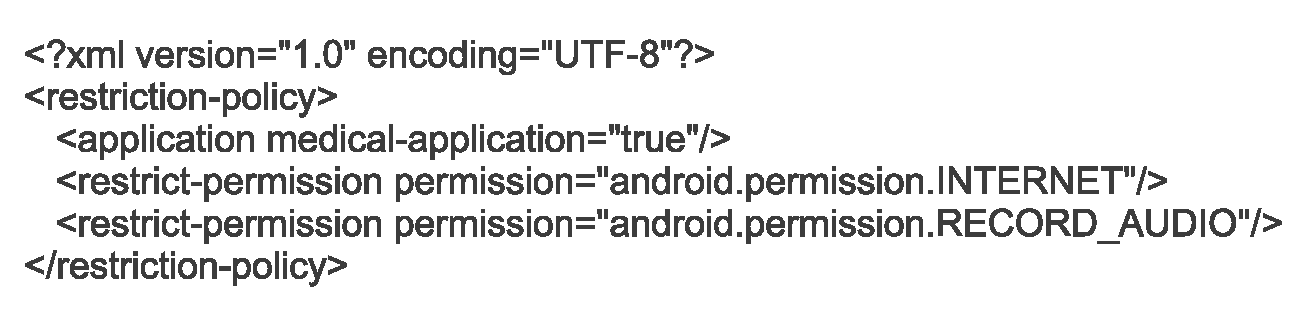
\psfig{file=restriction_policy.eps,width=3.0in}
\caption{An example of a policy restriction file.}
\label{fig:policy}
\end{figure}
%\vspace{-8mm}

\subsection{Dynamic Privilege Restrictions Implementation}

We implement a system service, named as Privilege Restriction Service (PRS),
which is responsible for enforcing and imposing the dynamic system-wide
privilege restrictions on applications.  PRS contains four hash maps to store
necessary information that DASF needs to enforce privilege restrictions on
applications, which store the following information:
 %The four hash maps store the following information.

\begin{itemize}
\item \textit{Medical application hash map:} Stores packages that are
 tagged as medical applications.
\item \textit{Requested permissions hash map:} Stores all of
the \textit{uses-permissions} that an application requests.
\item \textit{Restriction policy hash map:} Stores the privileges that
an application can programmatically restrict.
\item \textit{Restricted privileges hash map:} Stores the system-wide
permission restrictions currently imposed on applications.
\end{itemize}

We decide to store the package information in RAM rather than on flash memory
to prevent unauthorized modification of our framework data (e.g., pulling a
file via a USB connection, or changing the contents and then pushing it back to
the device). Furthermore, DASF can repopulate the hash maps if the device is
shutdown since Android reparses all of the installed packages during the boot
process, which makes main memory the ideal location to store our framework
data.  Moreover, the entries that are enforced by the server in the
\textit{restriction policy hash map} can be restored to its previous state
since our PRS communicates with the trusted server during the boot process.
PRS is started by the \textit{Service Manager} in Android during the booting.
When PRS starts, it communicates with the server to fetch the secret key needed
to decrypt security policies received from the server.   

We place a hook in Android's \textit{Package Parser} to parse the
\textit{restriction\_policy.xml} manifest file. When an application is
installed, the user is notified if the APK's restriction policy file includes
the \textit{medical application} tag and the restricted permissions policy that
it declares. For the application to continue installation, the user must
approve the policies declared in the restriction policy file.  Once the
policies are approved, a hook in the \textit{Package Manager Service} invokes
PRS to add the \textit{uses-permissions} that an application requests in its
manifest file to the \textit{requested permissions hash map}.  Furthermore, the
hook in the \textit{Package Manager Service} also invokes PRS to populate the
\textit{medical applications hash map} and the \textit{restriction policy hash
map} if the application included the \textit{restriction\_policy.xml} manifest
file.  We also restrict applications that are declared as \textit{medical
applications} from sharing a UID to ensure that they run in their own isolated
process and are the only application that may access their application's
directory and files.  Medical applications must have a unique UID because a
developer that creates a medical application could maliciously create a
different application signed with the same developer signature to access the
sensitive files of the medical application.

We provide a \textit{Privilege Restriction} class in the \textit{android.}
package that allows applications to programmatically enforce a privilege
restriction or unrestrict a previously restricted permission.  The application
can call the \textit{restrictPermission()} method with the permission name as
the argument of the method to restrict a permission.  The
\textit{restrictPermission()} method invokes PRS to check whether the
application that calls the method has requested to the restricted permission by
checking the \textit{restriction policy hash map}.  If the permission is in the
\textit{restriction policy hash map} under the calling application's entry, the
permission restriction is imposed by adding an entry to the \textit{restricted
privileges hash map} and all currently running applications that request that
permission are closed.  Furthermore, an application may unrestrict a previously
imposed permission restriction by calling the \textit{unrestrictPermission()}
method with the permission name as the argument of the method.  The
\textit{unrestrictPermission()} method invokes PRS to ensure that the
application attempting to unrestrict the permission is the one that imposes the
restriction.  If the application's UID matches the UID of the application that
imposed the restriction, the permission is unrestricted by removing the entry
from the \textit{restricted permissions hash map}.

We place hooks in the \textit{Activity Manager Service} so when an
application's component (e.g., activities, services, broadcast receivers, or
content providers) is attempting to start, our PRS is called to enforce the
security policies for starting applications as defined in our security model.

\subsection{Sensitive Data Security Policies Implementation}  

DASF allows an application developer to programmatically classify the
sensitivity level of data and also allows a server to classify the sensitivity
level of data that it sends to the device.  An application developer can
programmatically classify data by calling methods in the \textit{Data
Classification} class that DASF provides. For example, an application developer
can prevent a string containing PHI data from being written to the disk by
calling the \textit{preventDiskWrite()} method with the string as the argument.
The \textit{Data Classification} class also provides the following methods,
\textit{preventForwarding()} and \textit{preventDiskWriteAndForwarding()} to
enforce the security policies on data as discussed in our security model.
These methods add the corresponding privacy tag to the data.

%We place hooks in the Android system to enforce the security
%policies imposed on the sensitive data.  
To prevent data from being written to flash memory, we place a hook in the
\textit{Posix} class to enforce restrictions on data that is written to a file
and the \textit{SQLite} library to enforce restrictions on data that is written
to an SQLite database through insert and update statements.  These hooks check
the privacy tag of the data attempted to be written to flash memory and blocks
the operation if the privacy tag matches the tags that prevent disk writes.  
%We assume that the CleanOS SQLite patch for retaining privacy tags on
%retrievals from the database is implemented to ensure correct propagation of
%the privacy tags on individual entries.  
To prevent data from being forwarded from the device, we place hooks in the
\textit{Posix} class, the \textit{BluetoothSocket} class, and the
\textit{SmsManager} class to enforce whether PHI data is permitted to be sent
over a socket, a bluetooth connection, or through an SMS message.  These hooks
check the privacy tag of the data attempted to be forwarded from the device and
blocks forwarding the data if the privacy tag matches the tags that prevent
forwarding data.

\subsection{Message Protocol Implementation} 

As stated in our security model, our message protocol consists of two different
types of messages.  First, the \textit{data message} is used by the server to
send data and its corresponding sensitivity level to a medical application.
Second, the server may send a \textit{permission control message} to impose
system-level permission restrictions, or unrestrictions, on the device.
%Second, the server may prepend a \textit{permission control message} to a
%\textit{data message} to impose the system-level permission restrictions, or
%unrestrictions, on the device.

Whenever a medical application requests data from the server, the server
replies the application with the payload of a \textit{data message}.  The
\textit{data message} contains a 4-byte header and a payload.  The header
contains 1-bit to identify the type of message, 2-bits to identify the
sensitivity level that the server imposes on the payload, and  29-bits for the
length of the payload. Messages larger than $2^{29}$ bytes can be fragmented
and transmitted in multiple \textit{data messages}.
%Thus, the server can transmit $2^{29}$ bytes of data in
%one \textit{data message}.  However, if the server needs to transmit
%more than $2^{29}$ bytes of data, it can break the response up
%into multiple \textit{data messages}.

Further, the server may also prepend a \textit{permission control message} to
the \textit{data message}.  The \textit{permission control message} contains a
2-byte header, which contains 1-bit to identify the type of the message, 1-bit
to denote that a \textit{data message} is appended, and 14-bits for the length
of the payload.  Therefore, the server can transmit $2^{14}$ bytes of
permission restrictions and permission unrestrictions in one \textit{permission
control message}.

To force \textit{medical applications} to communicate with the trusted server,
we place a hook in the \textit{Posix} class to invoke PRS to determine whether
the application is a \textit{medical application} by checking whether or not
its UID is in the \textit{medical application hash map}.  If it is true, we
force the connection to the server through a tunnel that builds on either SSL
or IPsec. 

%changing the IP address to the server's
%IP address.  Again, we assume that the server will reject the connection
%if communication is not attempted over an SSL connection.

To ensure \textit{medical applications} use our protocol, which is transparent
to the application, we implement the protocol over an \textit{InputStream}
called the \textit{MessageInputStream}. When an application calls the
\textit{getInputStream()} method, the \textit{MessageInputStream} is returned
instead of the default input stream.

%The
%\textit{MessageInputStream} is returned when an application calls the
%\textit{getInputStream()} method instead of the default input stream.

Whenever an application receives a message from the server, the
\textit{MessageInputStream} first checks whether the message contains a
\textit{permission control message}.  If the message has a \textit{permission
control message} prepended to it, the \textit{MedicalInputStream} parses the
header and continues reading the length of the \textit{permission control
message's} payload.  After it receives the entire payload, it passes the
encrypted payload to the \textit{Privilege Restriction Service}.  PRS decrypts
the payload, enforces the requested permission restrictions as defined in our
security model, enforces the requested permission unrestrictions, and then
updates the secret key. If the \textit{data appended flag} is set in the
\textit{permission control message}, the \textit{MessageInputStream} reads the
header of the \textit{data message}, extracts the payload size, and the
sensitivity level of the payload.  Once the \textit{MessageInputStream} obtains
this information, it reads in the requested number of bytes, adds the
corresponding sensitivity level as the data's privacy tag, and returns the data
back to the application that requested the data.  This process is shown in
Fig.~\ref{fig:frameworkcomponents}. 

\begin{figure}[ht]
\centering
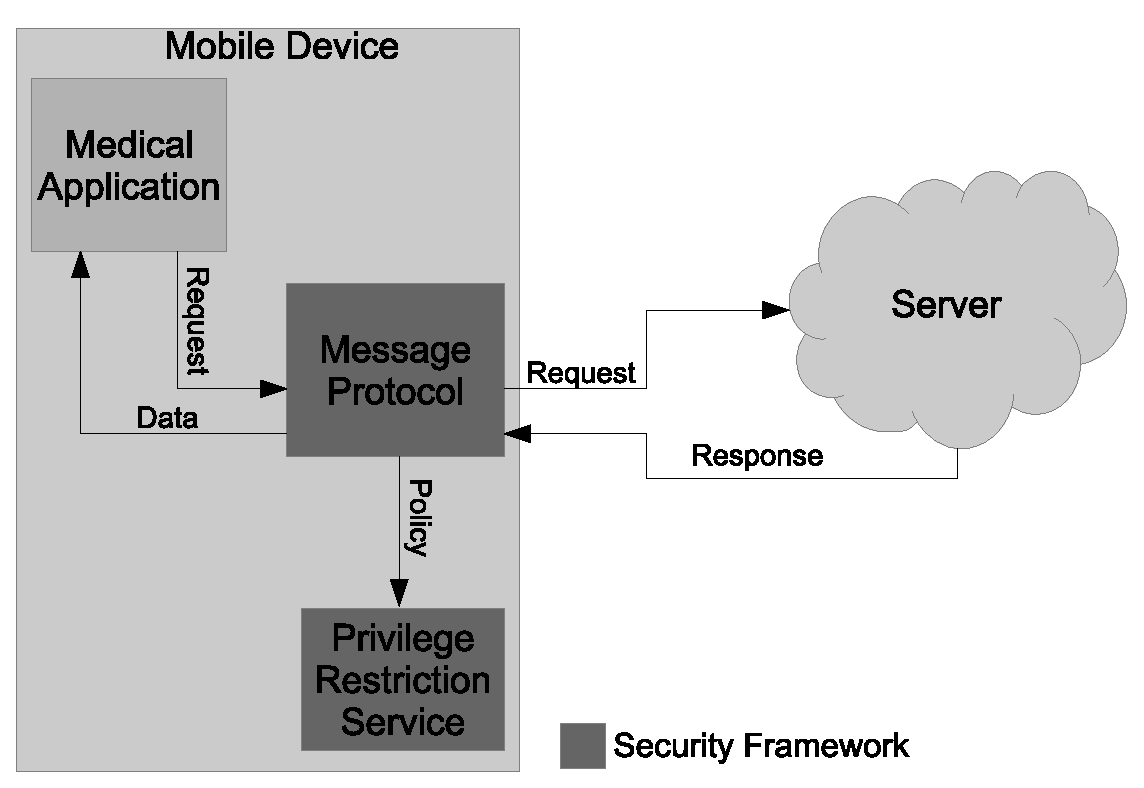
\psfig{file=frameworkcomponent.eps, width=2.5in}
\caption{Message Protocol Flow}
\label{fig:frameworkcomponents}
\end{figure}


